\documentclass[12pt]{article}
\usepackage[margin=0.5in]{geometry}
\usepackage{etoolbox}
\newtoggle{showAnswers}
\togglefalse{showAnswers}
%\toggletrue{showAnswers}% toggle this line to show/hide answers
\iftoggle{showAnswers}{ 
    \newenvironment{answer}{\vspace{1em}\color{blue!90!black}}{}
}{%
    \usepackage{verbatim}
    \newenvironment{answer}{\vspace{0em}\expandafter\comment}{\expandafter\endcomment} 
}%
\usepackage{xcolor}
\usepackage{amsfonts}
\usepackage{mathtools}
\usepackage[singlelinecheck=false]{caption}
\renewcommand\labelitemi{}% no bullets
\usepackage{sectsty}% smaller font for \section
    \sectionfont{\fontsize{12}{15}\selectfont}
\setlength\parindent{0pt}% no indents
\usepackage[colorlinks = true,
            linkcolor = black,
            urlcolor  = blue,
            citecolor = black,
            anchorcolor = black]{hyperref}
\usepackage{tikz}
\usetikzlibrary{calc}



\title{Ask Math Anything}
\author{Daily Challenge with Po-Shen Loh}
\date{23 June 2020}

\begin{document}
\begin{minipage}{\textwidth}
\maketitle
\begin{abstract}
Professor Po-Shen Loh solves problems on his YouTube channel. A selection for practice. 

Reference:~ 
\href{https://www.youtube.com/channel/UCf78EJOm4wQ4xXwSS15PuxQ}{Ask Math Anything - Daily Challenge with Po-Shen Loh}
\end{abstract}
\end{minipage}

\section*{2020/06/23}
\section{A Sum Problem}
Find $a$ and $b$ for
\begin{align*}
(3^{2006} + 2006)^2 - (3^{2006} - 2006)^2 = a^{b}
\end{align*}
\begin{answer}
Hint \#1: 
\begin{align*}
(a+b)^2 = (a+b)(a+b) 
  & = a \times a + a \times b + b \times a + b \times b \\
  & = a^2 + 2 ab + b^2
\end{align*}
Hint \#2:
\begin{align*}
(a-b)^2 = a^2 - 2 ab + b^2
\end{align*}
Hint \#3:
\begin{align*}
(a+b)^2 - (a-b)^2 =  4 ab
\end{align*}
Hint \#4:
\begin{align*}
4 \times 2006 \times 3^{2006}
\end{align*}
Hint \#5: Is $4 \times 2006$ a multiple of $3$?

\bigskip

If you enjoyed the previous problem, try this one:
\bigskip

Find $a$ and $b$ for
\begin{align*}
(3^{2019} + 2019)^2 - (3^{2019} - 2019)^2 = a^{b}
\end{align*}
\end{answer}


\section{A Sum Problem}
\begin{align*}
\frac{2020^2 - 2012^2}{2017^2 - 2015^2}
\end{align*}

\begin{answer}
Hint \#1:
\begin{align*}
\frac{a^2 - b^2}{c^2 - d^2}
= \frac{(a-b)(a+b)}{(c-d)(c+d)}
\end{align*}

Hint \#2:
\begin{align*}
\frac{4032 \times 8}{4032 \times 2} = 4 
\end{align*}
\end{answer}

\section{A Sum Problem}
Milly adds up all integers from $1$ to $n$ inclusive.
Billy adds up all integers from $n+1$ to $20$ inclusive.
They obtain the same sum. What is the value of $n$?

\begin{answer}
Let $S_{n}$ be the sum of all integers from $0$ to $n$. There is a well-known formula for this sum. That's the formula that, supposedly, schoolboy math genius Gauss used to calculate the sum of the first $100$ integers. 
\begin{align*}
S_{n} = 1 + 2 + \ldots + n
= \frac{n(n+1)}{2}
\end{align*}
\subsubsection*{Proof 1:}
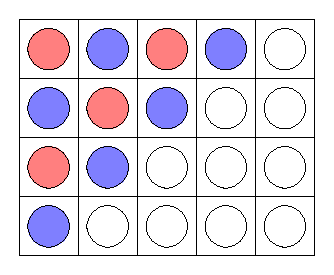
\includegraphics{tikz-matrix-nodes-circles-2}\bigskip\\
Count the circles along the diagonal starting from the top-left corner, adding circles of the same color at each step (red, then blue, then red, then blue). The sequence is $1$ (for $n=1$), $3$ (for $n=2$), $6$ (for $n=3$), $10$ (for $n=4$). This last number is the sum of the first $4$ integers. Denote it $S_{4}$,
\begin{align*}
S_{4} = 1 + 2 + 3 + 4
\end{align*}
By symmetry, there are also $10$ white circles. Thus the total number of circles in the matrix is $2 \times S_{4} = 20$. But clearly, this is also the ``area'' of the rectangle $20=4\times5$ (height times width). The argument is general and therefore $2 S_{n} = n(n+1)$. There are several other interesting proofs. 

\subsubsection*{Proof 2:}
Another popular proof is to rearrange the sum:
\begin{align*}
S_{n} & = 1 ~+~~~~2 ~~~~+~~~~3 ~~~~+~\ldots~ (n-1) ~+~ n \\
      & = n ~+ (n-1) + (n-2) + ~\ldots~~~~~ 2 ~~~~~ + ~ 1
\end{align*}
Now consider the terms that are aligned vertically: The first two add up to $1+n$. The next two add up to $2+(n-1)=1+n$. Next, $3+(n-2)=1+n$. And so on. Thus the sum $2S_{n}$ is equal to a repeated sum of  $(1+n)$. How many times is the sum repeated? From the first line, exactly $n$ repetitions. And thus,
\begin{align*}
2 S_{n} = (1+n) \times n
\end{align*}
\subsubsection*{Proof 3:}
Another way to prove this is a by induction: If $S_{n}=n(n+1)/2$, then $S_{n+1}=(n+1)(n+2)/2$. The statement clearly holds for $n=0$ since $S_{0} = 0 = 0 (0+1)/2$. Thus it must hold for every integer $n>0$. The ``If, then'' part can be proved like this:
\begin{align*}
S_{n+1} 
  & = ~~~~ S_{n} ~~~~+ (n+1) \\
  & = \frac{n(n+1)}{2} + (n+1) \\
  & = \frac{n(n+1)+2(n+1)}{2} \\
  & = \frac{(n+1)(n+2)}{2}
\end{align*}
\textit{Quod erat demonstrandum.} But let's get back to our problem.
\bigskip

Let $S_{20}$ be the sum of all integers from $0$ to $20$:
\begin{align*}
S_{20} = 1 + 2 + \ldots + 20 
= \frac{20(1+20)}{2}
= 210
\end{align*}
This number is partitioned between Milly and Billy.
\begin{align*}
S_{20} ~~ = ~~ \underbrace{~~~~S_{n}~~~~}_{\text{Milly}} ~~+~~ \underbrace{S_{20}-S_{n}}_{\text{Billy}}
\end{align*}
Milly and Billy obtain the same sum: 
\begin{align*}
S_{n} & = S_{20}-S_{n} \\
\Rightarrow ~~
2S_{n} & = S_{20} = 210 \\
\Rightarrow ~~
n (n+1) & = 210
\end{align*}
So now the problem boils down to finding two successive integers that multiplied together yield $210$. Clearly $n$ must be less than the square root of $210$, but not much less. In general, for any $n>0$, this inequality holds:
\begin{align*}
n^2 < n(n+1) < (n+1)^2
\end{align*}
This is where it is useful to have a few squares memorized. For instance,
\begin{align*}
1, 4, 9, 16, 25, 36, 49, 64, 81, 100, 121, 144, 169, 196, 225, 256, 289, 324, 361, 400, \ldots 
\end{align*}
Everybody knows $12^2=144$. Professor Po-Shen Loh knows them all! The solution is now obvious:
\begin{align*}
n  & \times (n+1) \\
= ~~ 14 & \times ~~~ 15
\end{align*}
Answer: $n=14$.
\end{answer}


\section{A Percentage Problem}
\begin{itemize}
\item $10\%$ of the students score $70$pts each. 
\item $35\%$ of the students score $80$pts each. 
\item $30\%$ of the students score $90$pts each. 
\item $25\%$ of the students score $100$pts each. 
\end{itemize}
What is the difference between the median and the mean?

\begin{answer}
First, we define these ``measures of dispersion''. The mean will be denoted $\mu$, the median $m$. 
The median $m$ is the value that divides the set such that half lie below and half above. In practice, the median may be found by throwing away the greatest and lowest values a pair at a time until there are either two values left or one value left. If the set has an even number of elements, there will be two values left (we can split the set exactly in two halves). If the set has an odd number of elements, there will be one value left (we cannot split the set exactly, there is an extra element that we must place arbitrarily above or below). In this problem, there are only $4$ possible scores, making it easy to identify the median. The data states that $10\%$ of the students have a score no more than $70$pts, $45\%$ have a score no more than $80$pts, $75\%$ have a score no more than $90$pts. The median score is therefore $m=90$pts. If we divide the class with students with score $70$pts and $80$pts on one side, and students with score $100$pts on the other side, we then can distribute $10\%$ of those students with score $90$pts into the lower group and the remaining $20\%$ into the higher group. How to choose the $90$-score students for this partition? At random, because we have no data to distinguish them! 

The arithmetic mean is the sum of all the scores for all the students divided by the total number of students. Let $n_1$ denote the number of students with score $s_1$, $n_2$ with score $s_2$, and so on. The mean is
\begin{align*}
\mu 
& = \frac{n_{1}s_{1}+n_{2}s_{2}+n_{3}s_{3}+n_{4}s_{4}}{n_{1}+n_{2}+n_{3}+n_{4}} \\ & \\
& = \frac{n_{1}s_{1}+n_{2}s_{2}+n_{3}s_{3}+n_{4}s_{4}}{n} \\ & \\
& = 
\left(\frac{n_{1}}{n}\right)s_{1} + \left(\frac{n_{2}}{n}\right)s_{2} + \left(\frac{n_{3}}{n}\right)s_{3} + \left(\frac{n_{4}}{n}\right)s_{4}
\end{align*}
where $n$ is the total number of students $n=n_{1}+n_{2}+n_{3}+n_{4}$. But these ratios are just percentages. That is, $p_{1}$ is the fraction of students who received score $s_{1}$,
\begin{align*}
p_{1} = \frac{n_{1}}{n}
\end{align*}
$p_{2}$ who received score $s_{2}$, and so on. Thus we can calculate the mean from data about the percentages and the scores:
\begin{align*}
\mu = p_{1}s_{1} + p_{2}s_{2} + p_{3}s_{3} + p_{4}s_{4}
\end{align*}
Using the data gives:
\begin{align*}
\mu 
& = 0.1 \times 70 + 0.35 \times 80 + 0.3 \times 90 + 0.25 \times 100 \\
& = 7 + 28 + 27 +  25 \\
& = 87
\end{align*}

\end{answer}

\end{document}